\documentclass[conference]{IEEEtran}
\IEEEoverridecommandlockouts
\usepackage[utf8]{inputenc}
\usepackage[T1]{fontenc}
\usepackage[spanish,es-noshorthands,es-tabla]{babel}
\usepackage{cite}
\usepackage{amsmath,amssymb}
\usepackage{graphicx}
\usepackage{booktabs}
\usepackage{url}
\usepackage[hidelinks]{hyperref}

\begin{document}

\title{TRM Predict: sistema de analítica predictiva nativo en la nube para decisiones ante el riesgo cambiario en Colombia}

\author{
\IEEEauthorblockN{Sebastián Cubides, Nicolás Vergara, Edgar Ruiz}
\IEEEauthorblockA{\textit{Ingeniería de Datos e Inteligencia Artificial, V semestre}\\
\textit{Universidad Santo Tomás}, Tunja, Colombia\\
Proyecto integrador: Minería de Datos, Machine Learning y Cloud Computing --- 2026-2}
}

\maketitle

\begin{abstract}
Los hogares colombianos que reciben remesas y las micro, pequeñas y medianas empresas (mipymes) importadoras están expuestos a la volatilidad de la tasa de cambio peso--dólar (TRM), pero no cuentan con las herramientas analíticas de las grandes empresas. Esta propuesta presenta \emph{TRM Predict}, un sistema de apoyo a decisiones nativo en la nube que pronostica, para el siguiente día hábil, la dirección de la TRM, su valor esperado y la probabilidad de un movimiento fuerte. El pipeline de datos sigue CRISP-DM e integra la TRM oficial (API de datos abiertos), variables de mercados globales, criptoactivos y un módulo de web scraping que convierte titulares de noticias financieras en un índice diario de sentimiento cambiario. La minería no supervisada (PCA, K-Means, clustering jerárquico, DBSCAN, Apriori y FP-Growth) caracteriza regímenes de mercado y reglas de co-movimiento. Los modelos supervisados van desde modelos lineales regularizados, KNN y SVM hasta ensembles (Random Forest, AdaBoost, Gradient Boosting), optimizados con Grid y Random Search bajo validación cruzada para series de tiempo y explicados con SHAP y LIME. El sistema se despliega en AWS con Terraform: una capa de ingesta serverless (EventBridge, Lambda), un data lake en S3 replicado a otra región, PostgreSQL en RDS y una API REST en contenedores detrás de un Application Load Balancer con auto-scaling en dos zonas de disponibilidad. El proyecto contribuye al ODS~8 (meta 8.10) y al ODS~10 (meta 10.c).
\end{abstract}

\begin{IEEEkeywords}
computación en la nube, minería de datos, aprendizaje automático, CRISP-DM, aprendizaje por ensambles, pronóstico de tasa de cambio, desarrollo sostenible
\end{IEEEkeywords}

\section{Introducción}
La \emph{Tasa Representativa del Mercado} (TRM) es la tasa de cambio oficial COP/USD que certifica a diario la Superintendencia Financiera de Colombia. De ella dependen el precio de los bienes importados, el valor de las remesas que reciben los hogares y el costo de la deuda en dólares. Entre septiembre de 2017 y octubre de 2026 la TRM se movió entre 2.705 (abril de 2018) y 5.061 COP/USD (noviembre de 2022). Solo en 2025 osciló entre 3.707 y 4.417, una variación del 19~\%. En nuestro conjunto de datos, el 18~\% de los días hábiles registra una variación superior al 1~\%.

Las grandes empresas gestionan este riesgo con mesas de tesorería y derivados; los hogares y las mipymes suelen decidir por intuición. Según el Banco de la República, las remesas hacia Colombia superaron los USD~11.800 millones en 2024~\cite{banrep_remesas}, de modo que incluso pequeñas mejoras en el \emph{momento} en que una familia convierte sus dólares representan ingresos significativos. Por ello el proyecto se alinea con la Agenda 2030 de las Naciones Unidas~\cite{un2015}: ODS~8 (meta 8.10, acceso a servicios financieros) y ODS~10 (meta 10.c, reducir el costo de las remesas).

\section{Planteamiento del problema}
\textbf{Problema.} Los agentes económicos no expertos en Colombia no disponen de una herramienta accesible, transparente y actualizada de forma continua para estimar el comportamiento y el riesgo de corto plazo de la TRM. \textbf{Usuarios.} (i) Hogares que reciben remesas; (ii) mipymes importadoras que deben comprar dólares; (iii) docentes y estudiantes de programas de educación financiera. \textbf{Pregunta.} Con datos públicos disponibles antes de la publicación de la siguiente TRM, ¿es posible (a) estimar la probabilidad de que suba, (b) estimar su valor esperado y (c) anticipar días con movimientos anormalmente fuertes, con un desempeño verificablemente mejor que líneas base ingenuas, y explicar cada predicción?

Las tasas de cambio son muy difíciles de pronosticar: Meese y Rogoff mostraron que los modelos estructurales no superan a un paseo aleatorio fuera de muestra~\cite{meese1983}. Por eso el proyecto adopta el paseo aleatorio y la clase mayoritaria como líneas base obligatorias, y privilegia el rigor y la evaluación honesta sobre la complejidad del modelo.

\section{Trabajos relacionados}
El aprendizaje automático aplicado a mercados financieros cuenta con revisiones extensas. Henrique \emph{et al.}~\cite{henrique2019} analizan más de 50 estudios y reportan que dominan las máquinas de vectores de soporte y las redes neuronales, con los ensembles ganando terreno. Sezer \emph{et al.}~\cite{sezer2020} revisan el aprendizaje profundo para series financieras y señalan la falta de interpretabilidad y reproducibilidad. La mayoría de estudios se enfoca en pares de monedas principales o índices bursátiles, rara vez en monedas emergentes como el peso colombiano, y pocos ofrecen un servicio desplegable y explicable para usuarios no expertos. Este proyecto cubre ese vacío combinando (i) determinantes propios de Colombia (petróleo, monedas pares de la región, sentimiento de noticias locales), (ii) ensembles interpretables con SHAP~\cite{lundberg2017} y LIME~\cite{ribeiro2016} y (iii) un despliegue en la nube reproducible con Infraestructura como Código.

\section{Sistema propuesto}
La Fig.~\ref{fig:arch} muestra el sistema de extremo a extremo. Cada día hábil a las 18:30 (hora de Colombia), después de publicada la TRM, una regla de EventBridge dispara una función Lambda de \emph{ingesta}. Esta consulta la API de datos abiertos de la TRM, Yahoo Finance (Brent, DXY, bono a 10 años de EE.~UU., VIX, S\&P~500, USD/MXN, USD/BRL y dólar spot USD/COP) y la API de Binance (BTC, ETH), y hace scraping de los titulares de \emph{La República}. El paquete JSON resultante llega a la zona \emph{raw} de un data lake en S3, y ese evento dispara una Lambda de \emph{ETL} que carga los registros en PostgreSQL. Los modelos se entrenan fuera de línea con el pipeline CRISP-DM y se publican en S3. Un servicio FastAPI en Docker carga el modelo y ofrece predicciones, escenarios hipotéticos y un tablero web.

\begin{figure*}[t]
\centering
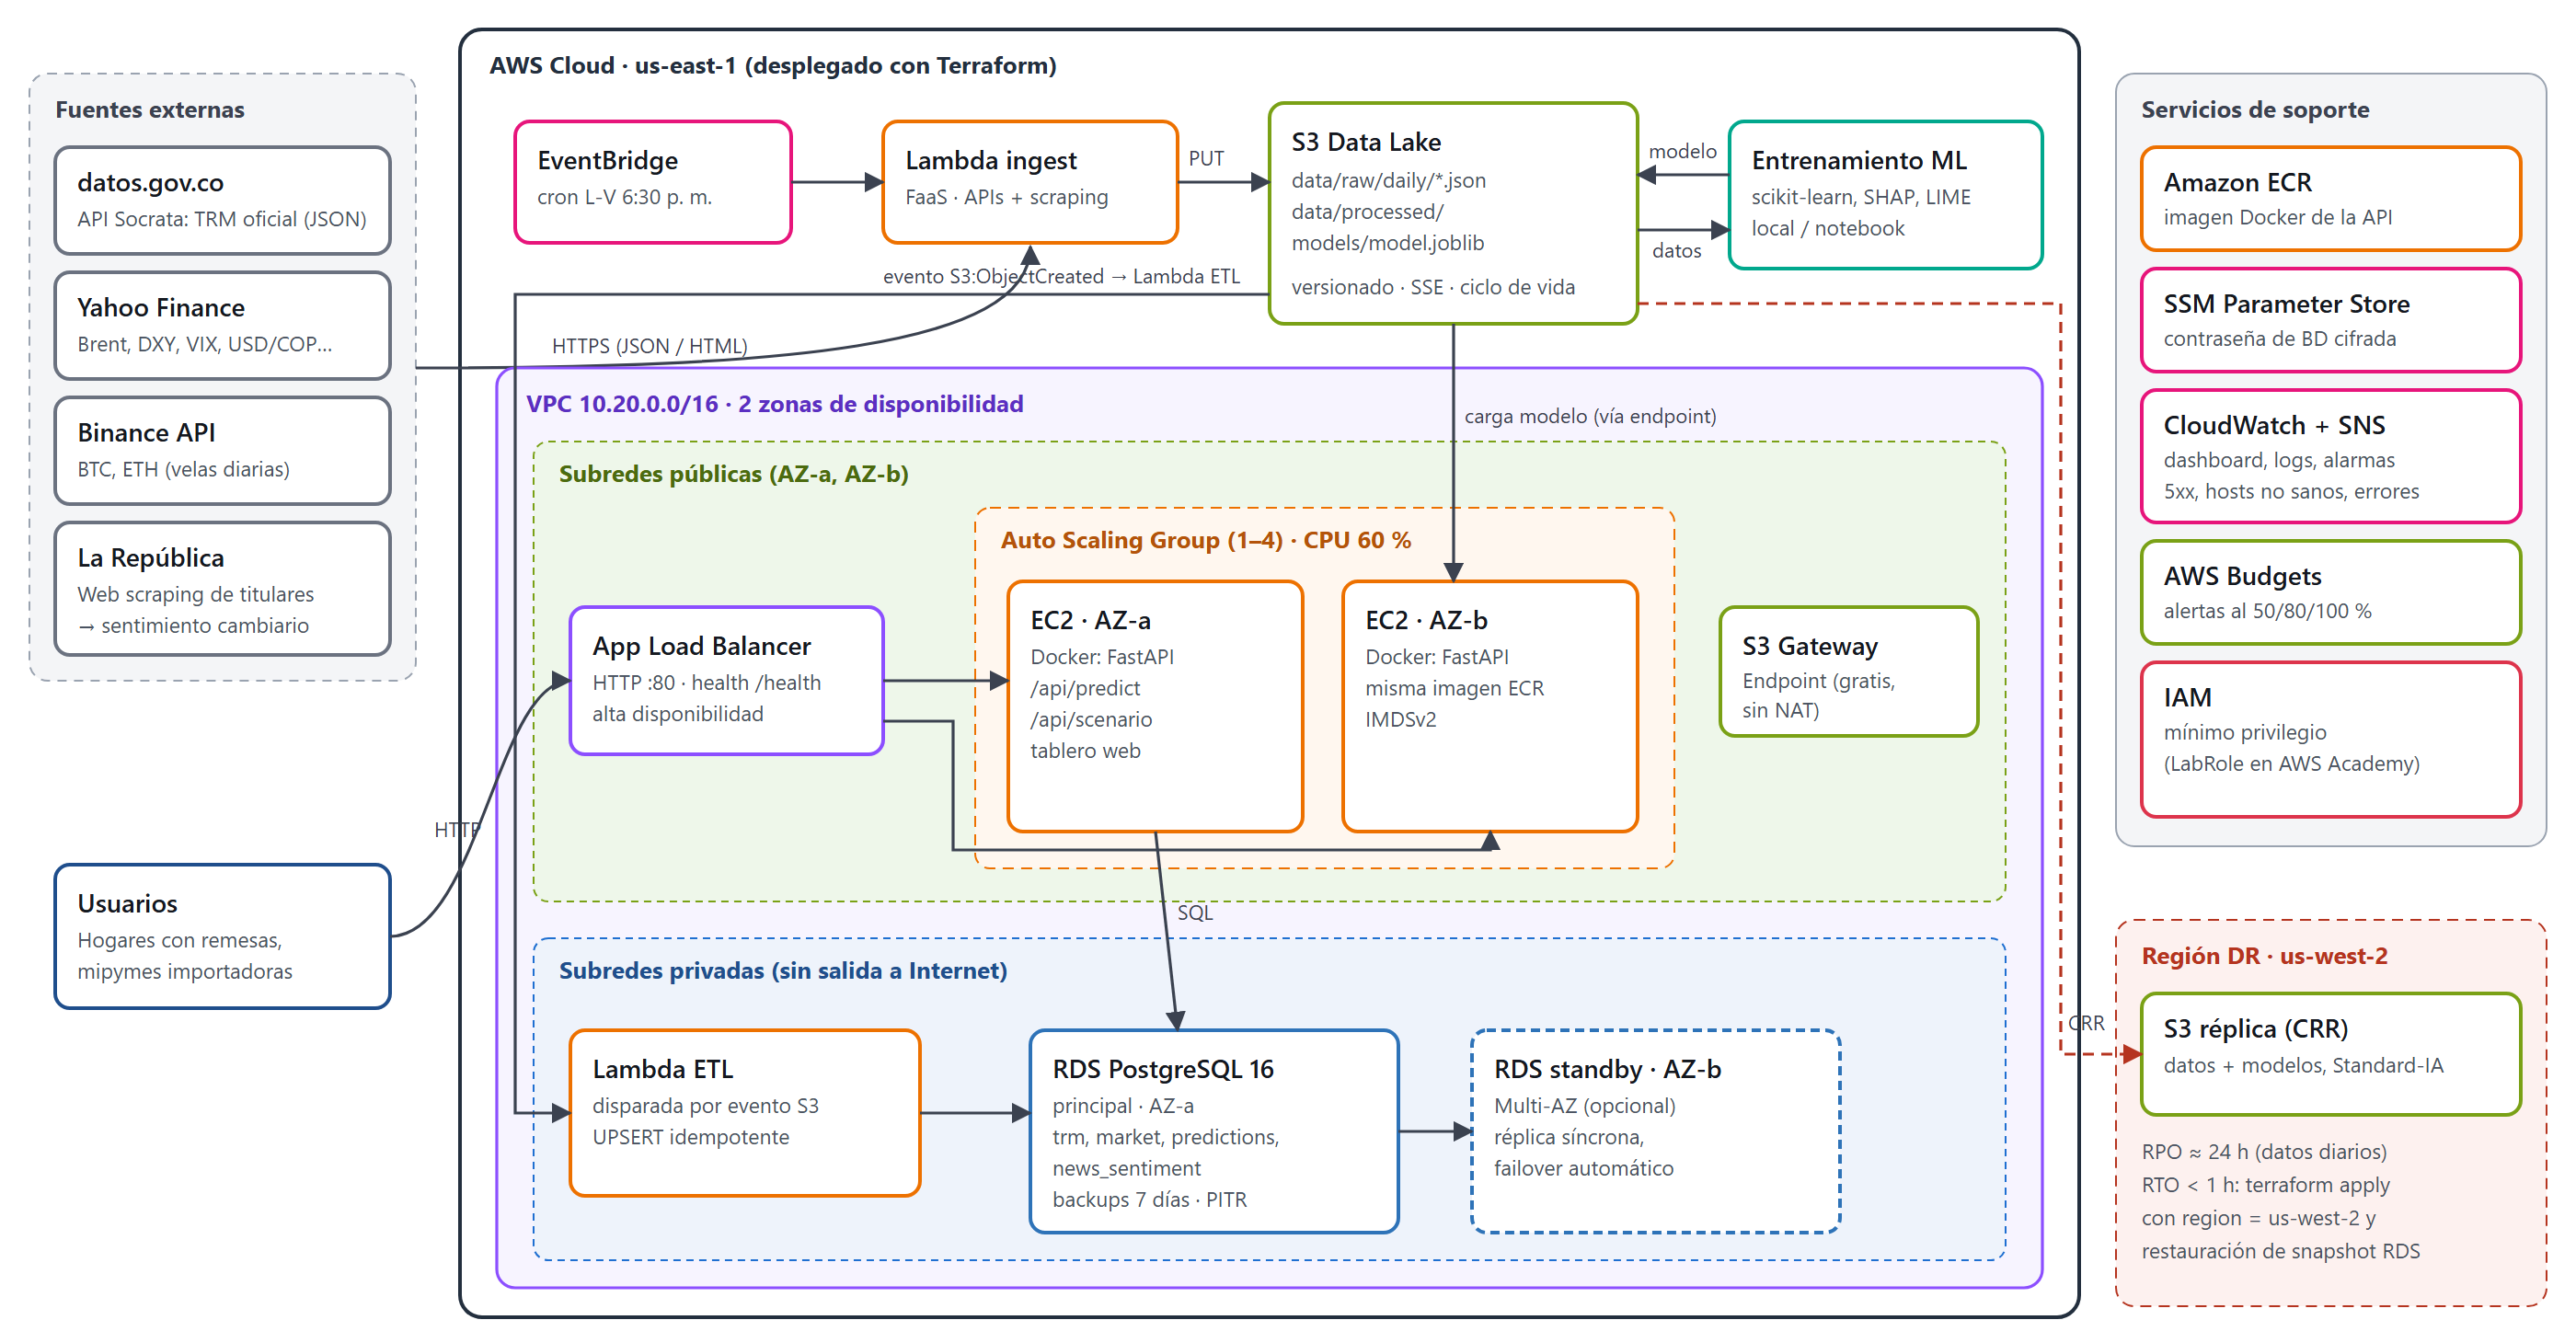
\includegraphics[width=\textwidth]{../arquitectura.png}
\caption{Arquitectura de TRM Predict en AWS: ingesta serverless, data lake en S3 con réplica entre regiones, RDS en subredes privadas y una API con auto-scaling detrás de un Application Load Balancer en dos zonas de disponibilidad.}
\label{fig:arch}
\end{figure*}

\section{Arquitectura en la nube}
\textbf{Proveedor y modelo de despliegue.} Nube pública en AWS (us-east-1), elegida por su alineación con el curso, los créditos de AWS Academy y la madurez de su proveedor de Terraform; una segunda región (us-west-2) se usa para recuperación ante desastres. \textbf{Modelos de servicio.} IaaS (instancias EC2 de la API), PaaS (RDS PostgreSQL, Application Load Balancer, ECR), FaaS (Lambda para ingesta y ETL) y SaaS (el tablero que consumen los usuarios finales), según las definiciones del NIST~\cite{nist800145}.

\textbf{Escalabilidad.} Un Auto Scaling Group (de 1 a 4 instancias \texttt{t3.micro}) con política \emph{target tracking} al 60~\% de CPU promedio; el almacenamiento de RDS crece automáticamente de 20 a 50~GB. \textbf{Alta disponibilidad.} El ALB abarca dos zonas de disponibilidad y solo enruta a instancias que superan el chequeo \texttt{/health}; el ASG reemplaza automáticamente las instancias no sanas; RDS puede operar en Multi-AZ con réplica síncrona y conmutación automática. \textbf{Recuperación ante desastres.} Versionado de S3 y réplica entre regiones (CRR) de datos y modelos; backups automáticos de RDS (7 días, recuperación a un punto en el tiempo); toda la plataforma puede reconstruirse en la región DR con \texttt{terraform apply}. Objetivos: RPO $\approx$ 24~h y RTO $<$ 1~h (estrategia \emph{backup and restore}~\cite{aws_wellarchitected}). \textbf{Seguridad.} RDS y la Lambda de ETL están en subredes privadas sin salida a Internet; S3 se accede mediante un VPC gateway endpoint gratuito (evita un NAT gateway); la contraseña de la base de datos se guarda cifrada en SSM Parameter Store; las instancias exigen IMDSv2 y solo aceptan tráfico del ALB. \textbf{IaC.} Todos los recursos (VPC, subredes, security groups, S3, RDS, ALB, ASG, Lambda, EventBridge, alarmas y tablero de CloudWatch, AWS Budgets) se declaran en Terraform~\cite{terraform_aws}, se versionan en el repositorio y se validan con \texttt{terraform validate}.

\section{Pipeline de minería de datos}
El pipeline sigue el proceso KDD~\cite{fayyad1996} organizado con CRISP-DM~\cite{wirth2000}. \textbf{Adquisición.} Cuatro fuentes y formatos heterogéneos: API Socrata en JSON (8.370 registros de TRM desde 1991), JSON de Yahoo Finance almacenado como CSV (8 series), JSON de Binance (2 criptoactivos) y scraping de HTML. El scraper tiene una función concreta: cuenta los titulares relacionados con el dólar y calcula un índice léxico de sentimiento cambiario, información cualitativa que ninguna API ofrece.

\textbf{Preparación.} Conversión de tipos, eliminación de duplicados y fechas inválidas, verificación de positividad, auditoría de atípicos de los retornos por rango intercuartílico y un \texttt{merge\_asof} estricto que solo usa datos de mercado publicados \emph{antes} de cada fecha de TRM, para evitar fuga de información. El conjunto final tiene 2.159 observaciones diarias (sep.~2017--oct.~2026) y 43 variables: retornos logarítmicos y rezagos de la TRM, volatilidad a 5 y 20 días, razón de medias móviles, z-score, variables de calendario, retornos a 1 y 5 días y volatilidad a 20 días de cada mercado, y la brecha entre la última cotización spot y la TRM vigente.

\textbf{EDA.} Estadísticas descriptivas, pruebas de distribución, mapas de calor de correlación y correlaciones móviles. Los retornos de la TRM son leptocúrticos (curtosis en exceso de 3,0; Jarque--Bera $p<10^{-100}$) y presentan autocorrelación positiva de primer orden (0,17), coherente con que la TRM es un promedio ponderado por volumen del día.

\textbf{Ingeniería de datos y minería no supervisada.} PCA requiere 26 de 43 componentes para conservar el 90~\% de la varianza: las variables son poco redundantes, y las dos primeras componentes representan el momentum del peso y de las monedas pares (PC1) y la volatilidad global (PC2). K-Means (con $k$ elegido por los métodos del codo y de la silueta, $k=3$) y el clustering jerárquico de Ward segmentan \emph{regímenes} de mercado (aversión al riesgo, apetito por riesgo y alta volatilidad). Los regímenes se traslapan (silueta 0,12), por lo que se usan como contexto y no como clases rígidas. DBSCAN~\cite{ester1996} marca 57 días anómalos (45 de ellos en 2020), en los que la volatilidad de la TRM del día siguiente es 1,7 veces mayor. Apriori~\cite{agrawal1994} y FP-Growth~\cite{han2000} sobre movimientos diarios discretizados producen reglas interpretables, por ejemplo \{Brent sube, DXY baja\} $\Rightarrow$ TRM baja (confianza 0,63; lift 1,22) y \{USD/BRL sube, USD/MXN sube, VIX sube\} $\Rightarrow$ TRM sube (confianza 0,60; lift 1,24).

\section{Modelo de machine learning}
Tres tareas supervisadas comparten la misma matriz de variables: (1) clasificación de la \emph{dirección} (la TRM sube o baja), (2) clasificación de \emph{riesgo} (el siguiente retorno absoluto supera el percentil 75 de entrenamiento) y (3) \emph{regresión} del siguiente retorno logarítmico, del que se deriva la TRM esperada. Todos los modelos son pipelines de scikit-learn~\cite{pedregosa2011} (escalado y, opcionalmente, selección de variables y expansión polinomial). Candidatos: regresión lineal, polinomial+Ridge, Ridge, Lasso y Elastic Net; regresión logística, KNN y SVM para clasificación; y los ensembles Random Forest~\cite{breiman2001}, AdaBoost~\cite{freund1997} y Gradient Boosting~\cite{friedman2001}. Los hiperparámetros se optimizan con \texttt{GridSearchCV} (modelos lineales, KNN, SVM, AdaBoost) y \texttt{RandomizedSearchCV}~\cite{bergstra2012} (Random Forest, Gradient Boosting) con \texttt{TimeSeriesSplit} de 5 pliegues. El modelo final se elige por el puntaje de validación cruzada, nunca por el de prueba, y luego se valora según su costo computacional e interpretabilidad. Las explicaciones globales usan TreeSHAP e importancia de variables; las explicaciones locales de la última predicción usan LIME.

\section{Metodología y plan de trabajo}
\textbf{Fases} (alineadas con las unidades de las asignaturas): F1 definición del problema y adquisición (semanas 1--3); F2 EDA e ingeniería de datos (4--6); F3 modelado y evaluación (7--10); F4 diseño en la nube y despliegue con IaC (8--12); F5 integración, análisis de costos, artículo IEEE y póster (13--16).
\textbf{Validación.} División cronológica 80/20 (periodo de prueba dic.~2024--oct.~2026), validación cruzada de series de tiempo y líneas base obligatorias: paseo aleatorio (RMSE) y clase mayoritaria (exactitud). Métricas: ROC-AUC, exactitud y F1 en clasificación; RMSE, MAE, $R^2$, razón de RMSE frente al paseo aleatorio y acierto direccional en regresión; silueta y Davies--Bouldin en clustering; soporte, confianza y lift en reglas; latencia, disponibilidad y costo en la capa de nube.
\textbf{Resultados preliminares.} Una primera ejecución completa (Tabla~\ref{tab:prelim}) muestra que solo los ensembles superan el azar en el periodo de prueba. En dirección, Random Forest y Gradient Boosting alcanzan un ROC-AUC de 0,55--0,57, frente a 0,47--0,50 de la regresión logística, KNN y SVM, lo que sugiere interacciones no lineales entre los determinantes. En la tarea de riesgo, los ensembles alcanzan un AUC de 0,59. El regresor Gradient Boosting reduce en 2,4~\% el RMSE del paseo aleatorio. La exactitud en dirección (53,2~\%) aún no supera a la clase mayoritaria (54,6~\%); cerrar esa brecha es el objetivo principal de la fase~3, mediante calibración de probabilidades, umbrales de decisión y la variable de sentimiento obtenida por scraping. Según SHAP, las variables más influyentes son la brecha spot--TRM, el último retorno de la TRM y la variación diaria del DXY.

\begin{table}[t]
\caption{Resultados preliminares en prueba (dic.~2024--oct.~2026, $n=432$)}
\label{tab:prelim}
\centering
\begin{tabular}{@{}lccc@{}}
\toprule
Modelo & AUC dir. & AUC riesgo & RMSE/PA \\
\midrule
Logística / Ridge & 0,497 & 0,549 & 0,997 \\
KNN & 0,474 & 0,571 & -- \\
SVM & 0,490 & 0,562 & -- \\
Random Forest & 0,555 & 0,585 & 0,987 \\
AdaBoost & 0,541 & 0,557 & -- \\
Gradient Boosting & \textbf{0,566} & \textbf{0,586} & \textbf{0,976} \\
\bottomrule
\end{tabular}
\end{table}

\textbf{Riesgos.} Baja predictibilidad de las tasas de cambio (se mitiga con líneas base honestas y la tarea de riesgo); cambios en la estructura de los sitios web (el scraper está aislado y sus fallas no detienen la ingesta numérica); restricciones de IAM en AWS Academy (Terraform admite el rol existente \texttt{LabRole}); sobrecostos (alertas de AWS Budgets y \texttt{terraform destroy} después de cada sesión).

\section{Resultados esperados}
(i) Un repositorio público con el pipeline CRISP-DM, los modelos entrenados, los scripts de Terraform y el conjunto de datos final; (ii) un sistema en vivo en AWS (API REST y tablero) con auto-scaling, conmutación por falla y réplica entre regiones demostrables; (iii) un informe del modelo con líneas base y explicaciones SHAP y LIME; (iv) el artículo final en formato IEEE en inglés y español y un póster A1; (v) un video de respaldo de la demostración.

\section{Uso de recursos y costos esperados}
La Tabla~\ref{tab:cost} resume el estimado mensual on-demand en us-east-1. Operar 24/7 costaría unos USD~64 al mes. Como la plataforma se crea y se destruye con Terraform, el costo esperado de todo el semestre (unas 40 horas de desarrollo, un día de pruebas de failover y una semana de operación continua para la sustentación) es de unos USD~21, dentro de los créditos de AWS Academy. Evitar el NAT gateway gracias al endpoint de S3 ahorra unos USD~33 al mes.

\begin{table}[t]
\caption{Costo mensual estimado (USD, on-demand, us-east-1, 24/7)}
\label{tab:cost}
\centering
\begin{tabular}{@{}lr@{}}
\toprule
Servicio (configuración) & USD/mes \\
\midrule
Application Load Balancer (tráfico bajo) & 17,0 \\
EC2: 2 $\times$ t3.micro + 16 GB gp3 & 16,5 \\
Direcciones IPv4 públicas (4) & 14,6 \\
RDS PostgreSQL db.t4g.micro + 20 GB & 14,0 \\
S3 + réplica entre regiones, ECR & 0,2 \\
Lambda, EventBridge, SSM & 0,0 \\
CloudWatch, transferencia de datos & 1,3 \\
\midrule
\textbf{Total (dev, Single-AZ)} & \textbf{63,6} \\
Producción (Multi-AZ, hasta 4 instancias) & 78--95 \\
\bottomrule
\end{tabular}
\end{table}

\begin{thebibliography}{99}
\bibitem{un2015} United Nations, ``Transforming our world: The 2030 Agenda for Sustainable Development,'' A/RES/70/1, 2015.
\bibitem{banrep_remesas} Banco de la Rep\'ublica de Colombia, ``Ingresos de remesas de trabajadores en Colombia,'' Estad\'isticas del sector externo, 2025. [En línea]. Disponible: \url{https://www.banrep.gov.co}
\bibitem{meese1983} R. A. Meese and K. Rogoff, ``Empirical exchange rate models of the seventies: Do they fit out of sample?'' \emph{J. Int. Econ.}, vol. 14, no. 1--2, pp. 3--24, 1983.
\bibitem{henrique2019} B. M. Henrique, V. A. Sobreiro, and H. Kimura, ``Literature review: Machine learning techniques applied to financial market prediction,'' \emph{Expert Syst. Appl.}, vol. 124, pp. 226--251, 2019.
\bibitem{sezer2020} O. B. Sezer, M. U. Gudelek, and A. M. Ozbayoglu, ``Financial time series forecasting with deep learning: A systematic literature review: 2005--2019,'' \emph{Appl. Soft Comput.}, vol. 90, Art. no. 106181, 2020.
\bibitem{lundberg2017} S. M. Lundberg and S.-I. Lee, ``A unified approach to interpreting model predictions,'' in \emph{Adv. Neural Inf. Process. Syst. (NeurIPS)}, vol. 30, 2017, pp. 4765--4774.
\bibitem{ribeiro2016} M. T. Ribeiro, S. Singh, and C. Guestrin, ```Why should I trust you?': Explaining the predictions of any classifier,'' in \emph{Proc. 22nd ACM SIGKDD Int. Conf. Knowl. Discov. Data Min.}, 2016, pp. 1135--1144.
\bibitem{nist800145} P. Mell and T. Grance, ``The NIST definition of cloud computing,'' NIST, Gaithersburg, MD, USA, Special Publication 800-145, 2011.
\bibitem{aws_wellarchitected} Amazon Web Services, ``Disaster recovery of workloads on AWS: Recovery in the cloud,'' AWS Whitepaper, 2021. [En línea]. Disponible: \url{https://docs.aws.amazon.com/whitepapers/latest/disaster-recovery-workloads-on-aws/}
\bibitem{terraform_aws} HashiCorp, ``Terraform AWS provider documentation,'' 2026. [En línea]. Disponible: \url{https://registry.terraform.io/providers/hashicorp/aws/latest/docs}
\bibitem{fayyad1996} U. Fayyad, G. Piatetsky-Shapiro, and P. Smyth, ``From data mining to knowledge discovery in databases,'' \emph{AI Mag.}, vol. 17, no. 3, pp. 37--54, 1996.
\bibitem{wirth2000} R. Wirth and J. Hipp, ``CRISP-DM: Towards a standard process model for data mining,'' in \emph{Proc. 4th Int. Conf. Pract. Appl. Knowl. Discov. Data Min.}, 2000, pp. 29--39.
\bibitem{ester1996} M. Ester, H.-P. Kriegel, J. Sander, and X. Xu, ``A density-based algorithm for discovering clusters in large spatial databases with noise,'' in \emph{Proc. 2nd Int. Conf. Knowl. Discov. Data Min. (KDD)}, 1996, pp. 226--231.
\bibitem{agrawal1994} R. Agrawal and R. Srikant, ``Fast algorithms for mining association rules,'' in \emph{Proc. 20th Int. Conf. Very Large Data Bases (VLDB)}, 1994, pp. 487--499.
\bibitem{han2000} J. Han, J. Pei, and Y. Yin, ``Mining frequent patterns without candidate generation,'' in \emph{Proc. ACM SIGMOD Int. Conf. Manag. Data}, 2000, pp. 1--12.
\bibitem{pedregosa2011} F. Pedregosa \emph{et al.}, ``Scikit-learn: Machine learning in Python,'' \emph{J. Mach. Learn. Res.}, vol. 12, pp. 2825--2830, 2011.
\bibitem{breiman2001} L. Breiman, ``Random forests,'' \emph{Mach. Learn.}, vol. 45, no. 1, pp. 5--32, 2001.
\bibitem{freund1997} Y. Freund and R. E. Schapire, ``A decision-theoretic generalization of on-line learning and an application to boosting,'' \emph{J. Comput. Syst. Sci.}, vol. 55, no. 1, pp. 119--139, 1997.
\bibitem{friedman2001} J. H. Friedman, ``Greedy function approximation: A gradient boosting machine,'' \emph{Ann. Statist.}, vol. 29, no. 5, pp. 1189--1232, 2001.
\bibitem{bergstra2012} J. Bergstra and Y. Bengio, ``Random search for hyper-parameter optimization,'' \emph{J. Mach. Learn. Res.}, vol. 13, pp. 281--305, 2012.
\end{thebibliography}

\end{document}
